% ------------------------------------------------------------------------------
% TYPO3 CMS 8 LTS - What's New - Chapter "Introduction" (Dutch Version)
%
% @author	Michael Schams <schams.net>
% @license	Creative Commons BY-NC-SA 3.0
% @link		http://typo3.org/download/release-notes/whats-new/
% @language	English
% ------------------------------------------------------------------------------
% LTXE-CHAPTER-UID:		7fdf26cc-362160ab-d6c8b905-19722b20
% LTXE-CHAPTER-NAME:	Introduction
% ------------------------------------------------------------------------------

\section{Inleiding}
\begin{frame}[fragile]
	\frametitle{Inleiding}

	\begin{center}\huge{\color{typo3darkgrey}\textbf{Inleiding}}\end{center}
	\begin{center}\large{\textit{Kort overzicht van de feiten}}\end{center}

\end{frame}

% ------------------------------------------------------------------------------
% LTXE-SLIDE-START
% LTXE-SLIDE-UID:		e0101f37-8bdf7907-cfb526e5-2dab7bef
% LTXE-SLIDE-ORIGIN:	344cc625-72176049-0721f1aa-0580f11a English
% LTXE-SLIDE-TITLE:		TYPO3 CMS 8 LTS - The Facts
% ------------------------------------------------------------------------------
\begin{frame}[fragile]
	\frametitle{Inleiding}
	\framesubtitle{TYPO3 v8 LTS}

	\begin{itemize}
		\item Publicatiedatum: 4 april 2017
		\item Publicatietype: LTS versie (Lang ondersteunde versie)
		\item Ontwikkeltijd: 18+ maanden
	\end{itemize}

	\begin{figure}
		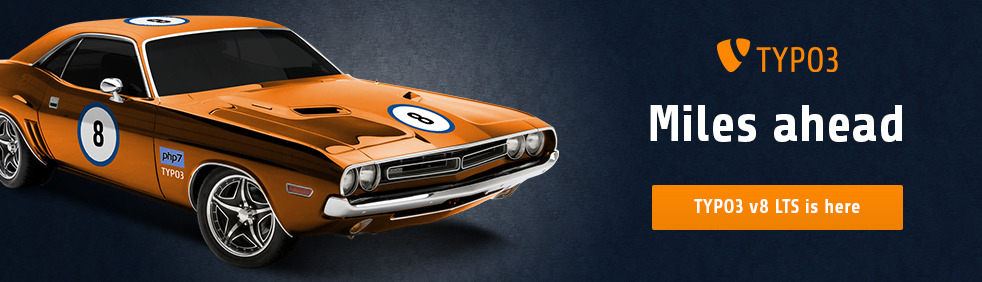
\includegraphics[width=0.95\linewidth]{Introduction/typo3cms87-banner.jpg}
	\end{figure}

\end{frame}

% ------------------------------------------------------------------------------
% LTXE-SLIDE-START
% LTXE-SLIDE-UID:		fe4dce56-c8381bba-c431635b-bdaa4049
% LTXE-SLIDE-ORIGIN:	59b04868-09a761b3-0c7ca4c3-ce6e31bb English
% LTXE-SLIDE-TITLE:		System Requirements (1)
% ------------------------------------------------------------------------------
\begin{frame}[fragile]
	\frametitle{Inleiding}
	\framesubtitle{Systeemeisen (1)}

%	\vspace{-0.2cm}
%	\begin{figure}\raggedleft
%		
\includegraphics[width=0.15\linewidth]{Introduction/logo-php7.png}
%	\end{figure}

	\begin{columns}[T]

		\begin{column}{.75\textwidth}
			\tabto{0.1cm}
				\begin{itemize}
					\item PHP 7.0 is de minimale versie\newline
						voor TYPO3 v8 LTS
					\item Volgende PHP 7 versies worden ondersteund zodra ze worden uitgebracht
					\item PHP 7 levert een significante snelheids winst
					\item Geeft de mogelijkheid om PHP 7 specifieke functies te gebruiken

				\end{itemize}
		\end{column}

        \begin{column}{.25\textwidth}
			
\includegraphics[width=0.5\linewidth]{Introduction/logo-php7.png}
        \end{column}

    \end{columns}

	\begin{itemize}
		\item Vereiste PHP instellingen:

			\begin{itemize}
				\item \texttt{memory\_limit} >= 128M
				\item \texttt{max\_execution\_time} >= 240s
				\item \texttt{max\_input\_vars} >= 1500
				\item compilatieoptie \texttt{-}\texttt{-disable-ipv6} \underline{niet} gebruiken
			\end{itemize}
	\end{itemize}


\end{frame}

% ------------------------------------------------------------------------------
% LTXE-SLIDE-START
% LTXE-SLIDE-UID:		7945f132-a4b2cab1-e397ddb5-f1be5517
% LTXE-SLIDE-ORIGIN:	ed65fc3f-293c3606-42f80134-5f1d7503 English
% LTXE-SLIDE-TITLE:		System Requirements (2)
% ------------------------------------------------------------------------------
\begin{frame}[fragile]
	\frametitle{Inleiding}
	\framesubtitle{Systeemeisen (2)}

	\begin{itemize}
		\item TYPO3 v8 LTS gebruikt \textbf{Doctrine DBAL}. Alle database servers
			die door deze database abstractie laag worden ondersteund, worden ook door TYPO3 ondersteund.\newline
			Bijvoorbeeld:
	\end{itemize}

	\vspace{-0.4cm}
	\begin{figure}
		
\includegraphics[width=0.70\linewidth]{Introduction/logo-databases.png}
	\end{figure}

	\begin{itemize}

		\item Minimaal benodigde schijfruimte: 200 MB
		\item De backend vereist Microsoft Internet Explorer 11 of hoger,
			Microsoft Edge, Google Chrome, Firefox, Safari
			of een andere moderne, compatibele browser

	\end{itemize}

\end{frame}


% ------------------------------------------------------------------------------
% LTXE-SLIDE-START
% LTXE-SLIDE-UID:		12fe7965-16b3357b-5184b6fc-bf5a46a8
% LTXE-SLIDE-ORIGIN:	41f1b51a-6b837f9d-c4aa9584-66f8e47f English
% LTXE-SLIDE-TITLE:		Sprint Releases
% ------------------------------------------------------------------------------
\begin{frame}[fragile]
	\frametitle{Inleiding}
	\framesubtitle{Ontwikkelings tijdlijn}

	Gepubliceerde sprint-releases:

	\begin{itemize}
		\item v8.0 \tabto{1.1cm}22 mar 2016\tabto{3.4cm}Lastminute toevoegingen
		\item v8.1 \tabto{1.1cm}03 mei 2016\tabto{3.4cm}Cloud-integratie
		\item v8.2 \tabto{1.1cm}05 jul 2016\tabto{3.4cm}Randvoorwaarden Doctrine
		\item v8.3 \tabto{1.1cm}30 aug 2016\tabto{3.4cm}Rich Text Editor
		\item v8.4 \tabto{1.1cm}18 okt 2016\tabto{3.4cm}Doctrine-migratie + upgrades
		\item v8.5 \tabto{1.1cm}20 dec 2016\tabto{3.4cm}Nieuwe RTE + Integrator-ondersteuning
		\item v8.6 \tabto{1.1cm}14 feb 2017\tabto{3.4cm}Polijsten
		\item v8.7 \tabto{1.1cm}04 apr 2017\tabto{3.4cm}Voorbereiding LTS
	\end{itemize}

\end{frame}

% ------------------------------------------------------------------------------
% LTXE-SLIDE-START
% LTXE-SLIDE-UID:		69d13e78-ee5511b0-685973ce-d0d817fd
% LTXE-SLIDE-ORIGIN:	f7c981ac-f359aac8-f8799a73-2adc6532 English
% LTXE-SLIDE-TITLE:		LTS Support Timeline
% ------------------------------------------------------------------------------
\begin{frame}[fragile]
	\frametitle{Inleiding}
	\framesubtitle{Lange Termijn Support}

	Onderhoud/support tijdlijn:

	\begin{figure}
		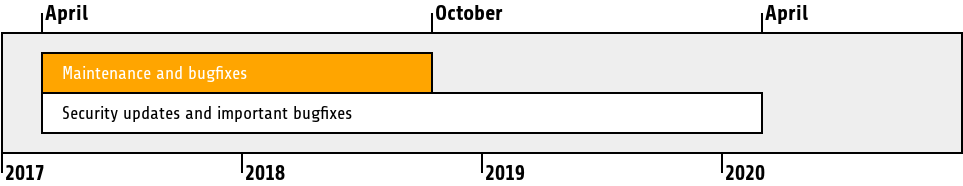
\includegraphics[width=1\linewidth]{Introduction/maintenance-support-timeline.png}
	\end{figure}

	\begin{itemize}
		\item TYPO3 versie 8.7 is een LTS Release (Lange Termijn Support)
		\item Regulier onderhoud en oplossen van algemene problemen tot oktober 2018
		\item Beveiliging en kritieke probleemoplossingen tot april 2020
	\end{itemize}

\end{frame}

% ------------------------------------------------------------------------------
